% ---------------------------------------------------------------------------------------------------------------
% TEMPLATE EM LATEX PARA TRABALHO DE CONCLUSÃO DE CURSO DA URI ERECHIM
% (ESTE TEMPLATE NÃO É UM PROJETO OFICIAL DA URI) CONSULTE SEU ORIETADOR CASO QUEIRA UTILIZA-LO
% Este template foi baseado no template da Universidade Tecnológica Federal do Paraná UTFPR
%
% Template baseado no projeto: http://tcc.tsi.gp.utfpr.edu.br/paginas/modelos-latex-da-utfpr
%
%----------------------------------------------------------------------------------------------------------------
% Codificação: UTF-8
% LaTeX:  abnTeX2
% ---------------------------------------------------------------------------------------------------------------

% CARREGA CLASSE PERSONALIZADA COM AS NORMAS DA URI-----------------------------------------------------------
\documentclass[oneside]{configs/uri-abntex2} %oneside -> impressão apenas frente

% INCLUI ARQUIVOS DE CONFIGURAÇÕES-------------------------------------------------------------------------------
% REFERÊNCIAS------------------------------------------------------------------
\usepackage[%
    alf,
    abnt-emphasize=bf,
    bibjustif,
    recuo=0cm,
    abnt-url-package=url,       % Utiliza o pacote url
    abnt-refinfo=yes,           % Utiliza o estilo bibliográfico abnt-refinfo
    abnt-etal-cite=3,
    abnt-etal-list=3,
    abnt-thesis-year=final
]{abntex2cite}                  % Configura as citações bibliográficas conforme a norma ABNT

% PACOTES----------------------------------------------------------------------
\usepackage[utf8]{inputenc}                                 % Codificação do documento
\usepackage[T1]{fontenc}                                    % Seleção de código de fonte
\usepackage{booktabs}                                       % Réguas horizontais em tabelas
\usepackage{color, colortbl}                                % Controle das cores
\usepackage{float}                                          % Necessário para tabelas/figuras em ambiente multi-colunas
\usepackage{graphicx}                                       % Inclusão de gráficos e figuras
\usepackage{icomma}                                         % Uso de vírgulas em expressões matemáticas
\usepackage{indentfirst}                                    % Indenta o primeiro parágrafo de cada seção
\usepackage{microtype}                                      % Melhora a justificação do documento
\usepackage{multirow, array}                                % Permite tabelas com múltiplas linhas e colunas
\usepackage{subeqnarray}                                    % Permite subnumeração de equações
\usepackage{lastpage}                                       % Para encontrar última página do documento
\usepackage{verbatim}                                       % Permite apresentar texto tal como escrito no documento, ainda que sejam comandos Latex
\usepackage{amsfonts, amssymb, amsmath}                     % Fontes e símbolos matemáticos
%\usepackage[algoruled, portuguese]{algorithm2e}             % Permite escrever algoritmos em português
%\usepackage[scaled]{helvet}                                % Usa a fonte Helvetica
\usepackage{times}                                          % Usa a fonte Times
%\usepackage{palatino}                                      % Usa a fonte Palatino
%\usepackage{lmodern}                                       % Usa a fonte Latin Modern
% \usepackage[bottom]{footmisc}                               % Mantém as notas de rodapé sempre na mesma posição
\usepackage{ae, aecompl}                                    % Fontes de alta qualidade
\usepackage{latexsym}                                       % Símbolos matemáticos
\usepackage{lscape}                                         % Permite páginas em modo "paisagem"
%\usepackage{picinpar}                                      % Dispor imagens em parágrafos
%\usepackage{scalefnt}
\usepackage{setspace}                                    % Permite redimensionar tamanho da fonte
%\usepackage{subfig}                                        % Posicionamento de figuras
%\usepackage{upgreek}                                       % Fonte letras gregas
\usepackage{listings}
\usepackage{nameref}                                        % Permite que o texto seja exibido ao invés do número numa referência (Ex.: \nameref{chap:introducao})

% Redefine a fonte para uma fonte similar a Arial (fonte Helvetica)
% \renewcommand*\familydefault{\sfdefault}
% Configura todo o documento para times new roman
\renewcommand{\familydefault}{ptm}

% CONFIGURAÇÕES DE APARÊNCIA DO PDF FINAL--------------------------------------
\makeatletter
\hypersetup{%
    portuguese,
    colorlinks=true,   % true: "links" coloridos; false: "links" em caixas de texto
    linkcolor=black,    % Define cor dos "links" internos
    citecolor=black,    % Define cor dos "links" para as referências bibliográficas
    filecolor=black,    % Define cor dos "links" para arquivos
    urlcolor=black,     % Define a cor dos "hiperlinks"
    breaklinks=true,
    pdftitle={\@title},
    pdfauthor={\@author},
    pdfkeywords={abnt, latex, abntex, abntex2}
}
\makeatother

% ALTERA O ASPECTO DA COR AZUL--------------------------------------------------
\definecolor{blue}{RGB}{41,5,195}

% REDEFINIÇÃO DE LABELS---------------------------------------------------------
\renewcommand{\algorithmautorefname}{Algoritmo}
\def\equationautorefname~#1\null{Equa\c c\~ao~(#1)\null}

% CRIA ÍNDICE REMISSIVO---------------------------------------------------------
\makeindex

% HIFENIZAÇÃO DE PALAVRAS QUE NÃO ESTÃO NO DICIONÁRIO---------------------------
\hyphenation{%
    qua-dros-cha-ve
    Kat-sa-gge-los
}

%%-----------------------------------------------------------------------------
%% VARIÁVEIS
%%-----------------------------------------------------------------------------
%% Utilize este arquivo para colocar valores que serão útes durante todo o
%%  documento (tal como a versão de um sistema ou o nome de uma ferramenta).

% Adaptive-DSD (singular, itálico)
\newcommand{\adaptive}{\textit{Adaptive-DSD} }

% Contêiner (singular, itálico)
\newcommand{\conteiner}{\textit{contêiner}}

% Containers (plural, itálico)
\newcommand{\containers}{\textit{containers}}

% Docker (itálico)
\newcommand{\docker}{\textit{docker}}

% Docker Network (itálico)
\newcommand{\dockerNetwork}{\textit{docker network}}

% GIT (itálico)
\newcommand{\git}{\textit{GIT}}

% Hangouts (itálico)
\newcommand{\hangouts}{\textit{Hangouts}}

% On-line (itálico)
\newcommand{\online}{\textit{on-line}}

% Software (itálico)
\newcommand{\software}{\textit{software}}

% Trello (itálico)
\newcommand{\trello}{\textit{Trello}}

% Web (itálico)
\newcommand{\web}{\textit{web}}





%%-----------------------------------------------------------------------------
%% COMANDOS
%%-----------------------------------------------------------------------------
%% Os comandos abaixo foram úteis em alguma situação e, para facilitar, foram
%%  colocados neste arquivo para centralizar sua definição.

% Insere aspas duplas acerca de um texto qualquer
\newcommand{\aspas}[1]{``#1''}

% Python style for highlighting
\newcommand\pythonstyle{\lstset{
    language=Python,
    basicstyle=\footnotesize,
    numbers=left,                   
    numberstyle=\tiny\color{gray},  
    stepnumber=1,                             
    numbersep=5pt,                  
    backgroundcolor=\color{white},    
    showspaces=false,               
    showstringspaces=false,         
    showtabs=false,                 
    frame=single,                   
    rulecolor=\color{black},        
    tabsize=2,                      
    captionpos=b,                   
    breaklines=true,                
    breakatwhitespace=false,
    keywordstyle=\color{blue},          
    commentstyle=\color{dkgreen},       
    stringstyle=\color{mauve}          
}}

% Python environment
\lstnewenvironment{python}[1][]
{
\pythonstyle
\lstset{#1}
}
{}

%%-----------------------------------------------------------------------------
%% CORES
%%-----------------------------------------------------------------------------
%% Cores definidas para apresentação de código fonte
\definecolor{dkgreen}{rgb}{0,0.6,0}
\definecolor{gray}{rgb}{0.5,0.5,0.5}
\definecolor{mauve}{rgb}{0.58,0,0.82}


% INCLUI ARQUIVOS DO DESENVOLVIMENTO DO DOCUMENTO (PRÉ-TEXTUAIS, TEXTUAIS, PÓS-TEXTUAIS)-----------------------

% INSERE CAPA
% CAPA---------------------------------------------------------------------------------------------------

% ORIENTAÇÕES GERAIS-------------------------------------------------------------------------------------
% Caso algum dos campos não se aplique ao seu trabalho, como por exemplo,
% se não houve coorientador, apenas deixe vazio.
% Exemplos: 
% \coorientador{}
% \departamento{}

% DADOS DO TRABALHO--------------------------------------------------------------------------------------
% \titulo{\textit{SkillBoard}: \\Sistema para candidatos encontrarem vagas e empresas gerenciarem processos de seleção}
\titulo{\textit{GerenciaDocker}: \\Sistema para gerenciar contêineres}

\titleabstract{Title in English}
\autor{João Vitor Veronese Vieira \\Kelwin Komka \\Vinicius Emanoel Andrade}
\autorcitacao{VIEIRA, João Vitor Veronese and KOMKA, Kelwin and ANDRADE, Vinicius Emanoel} % Sobrenome em maiúsculo
\local{ERECHIM - RS}
\data{2019}

% NATUREZA DO TRABALHO-----------------------------------------------------------------------------------
% Opções: 
% - Projeto de Conclusão de Curso (Disciplina de Projeto)
% - Trabalho de Conclusão de Curso (se for Graduação)
% - Dissertação (se for Mestrado)
% - Tese (se for Doutorado)
% - Projeto de Qualificação (se for Mestrado ou Doutorado)
\projeto{Trabalho de Conclusão de Curso}

% TÍTULO ACADÊMICO---------------------------------------------------------------------------------------
% Opções:
% - Bacharel ou Tecnólogo (Se a natureza for Trabalho de Conclusão de Curso)
% - Mestre (Se a natureza for Dissertação)
% - Doutor (Se a natureza for Tese)
% - Mestre ou Doutor (Se a natureza for Projeto de Qualificação)
\tituloAcademico{Bacharel}

% ÁREA DE CONCENTRAÇÃO E LINHA DE PESQUISA---------------------------------------------------------------
% Se a natureza for Trabalho de Conclusão de Curso, deixe ambos os campos vazios
% Se for programa de Pós-graduação, indique a área de concentração e a linha de pesquisa
\areaconcentracao{}
\linhapesquisa{}

% DADOS DA INSTITUIÇÃO-----------------------------------------------------------------------------------
% Se a natureza for Trabalho de Conclusão de Curso, coloque o nome do curso de graduação em "programa"
% Formato para o logo da Instituição: \logoinstituicao{<escala>}{<caminho/nome do arquivo>}
\instituicao{Universidade Regional Integrada do Alto Uruguai e das Missões Campus de Erechim}
\departamento{Departamento de Engenharias e Ciência da Computação}
\programa{Curso de Ciência da Computação}
\disciplina{Laboratório de Desenvolvimento}
%\logoinstituicao{0.2}{resources/figuras/logo-instituicao.png} 

% DADOS DOS ORIENTADORES---------------------------------------------------------------------------------
\orientador{Nome do orientador}
%\orientador[Orientadora:]{Nome da orientadora}
\instOrientador{Instituição do orientador}

\coorientador{Nome do coorientador}
%\coorientador[Coorientadora:]{Nome da coorientadora}
\instCoorientador{Instituição do coorientador}




% <START>
%   Conteúdo do Documento: base teórica.
% </START>
\begin{document}

    \pretextual
    \imprimircapa                                              	            % Comando para imprimir Capa
    
    % INSERE ELEMENTOS PRÉ-TEXTUAIS
    % SUMÁRIO----------------------------------------------------------------------

\renewcommand{\contentsname}{SUMÁRIO}

\pdfbookmark[0]{\contentsname}{toc}
\tableofcontents*
\cleardoublepage

% OBSERVAÇÕES-------------------------------------------------------------------
% Este arquivo não precisa ser alterado, pois o sumário é gerado automaticamente.
               			        % Sumário
    % Lista de Figuras----------------------------------------------------------------

\pdfbookmark[0]{\listfigurename}{lof}
\listoffigures*
\cleardoublepage

% OBSERVAÇÕES---------------------------------------------------------------------
% Este arquivo não precisa de ser alterado, pois a lista é gerada automaticamente.
           			        % Lista de Figuras

    \textual
    
    % INSERE ELEMENTOS TEXTUAIS
    % DESCRIÇÃO DO PROBLEMA-------------------------------------------------------------------

\chapter{DESCRIÇÃO DO PROBLEMA}
\label{chap:descricao_do_problema}

Em virtude da dinamicidade e agilidade necessárias em tarefas comuns para uma empresa de \software{}, tal como a disponibilização de aplicações para clientes ou mesmo a configuração de ambiente para novos colaboradores na equipe de desenvolvimento, criou-se o conceito técnico de \textit{conteinerização}. De modo resumido, esse conceito pode ser descrito, segundo \cite{Fernandes18}, como \aspas{o processo de distribuir uma aplicação de \software{} de maneira compartimentada, portátil e autossuficiente}. Isto é, uma forma de criar um ambiente completo de qualquer aplicação desenvolvida e \aspas{empacotá-lo}, para posteriormente distribuí-lo e utilizá-lo. 

Dentro desse cenário e tendo em vista os diversos benefícios que essa prática traz aos seus utilizadores, diversas ferramentas foram criadas. No entanto, um \software{} em específico acabou destacando-se como o mais utilizado quando se deseja implantar essa tecnologia. O \textbf{\docker{}} permite o gerenciamento completo de todos os \containers{} criados e, devido às suas funcionalidades, ganhou notoriedade na comunidade. 

No entanto, a utilização diária dessa ferramenta, geralmente realizada através de um terminal, pode se tornar uma tarefa desnecessária e até mesmo complicada, principalmente para um profissional iniciante, pois seu ambiente pode conter diversas especificidades (tal como vários \containers{} executando em paralelo) que, quando se está aprendendo a utilizar a ferramenta, podem ser difíceis de serem implementadas.

Além disso, vale ressaltar que, se necessário, o usuário deve controlar a rede (\dockerNetwork{}) em que os \containers{} estão sendo executados, o que acaba gerando ainda mais dificuldades. Com isso, fica nítido que, apesar de ser um recurso que proporciona inúmeras vantagens aos usuários, ainda existe uma barreira de adoção à essa tecnologia, principalmente em um contexto organizacional, pois o profissional que se dispõe a aprender essa nova ferramenta, precisará conciliar esse aprendizado com a realização de todas as demais atividades tradicionais que ele é encarregado.





% JUSTIFICATIVA-------------------------------------------------------------------
\section{Justificativa}
\label{sec:justificativa}

Baseando-se nos motivos descritos no capítulo \ref{chap:descricao_do_problema} e com o desejo de aprender mais sobre essa moderna ferramenta, o grupo considerou que um monitor \web{} que abstraísse essas dificuldades de gerenciamento em uma interface intuitiva e amigável para o usuário seria, além de uma ferramenta útil para os profissionais que se enquadram nessa situação, um bom assunto para ser o tema deste projeto.          		            % Descrição do Problema & Justificativa
    % OBJETIVOS-------------------------------------------------------------------

\chapter{OBJETIVOS}
\label{chap:objetivos}




\section{Objetivo Geral}
\label{sec:objetivo_geral}

\begin{itemize}
    \item Criar uma ferramenta que possibilite gerenciar os \containers{} em execução na máquina
\end{itemize}




\section{Objetivos Específicos}
\label{sec:objetivos_especificos}

\begin{itemize}
    \item Tornar a ferramenta flexível, permitindo que o usuário escolha o sistema operacional do \conteiner{} (com 4 opções)
    \item Construir uma interface amigável e intuitiva para o usuário
    \item Executar corretamente o algoritmo (\adaptive{}), que detectará falha nos \containers{}
\end{itemize}                  		            % Objetivos
    % METODOLOGIA-------------------------------------------------------------------

\chapter{METODOLOGIA}
\label{chap:metodologia}                 		            % Metodologia
    % FERRAMENTAS UTILIZADAS-------------------------------------------------------------------

\chapter{FERRAMENTAS UTILIZADAS}
\label{chap:ferramentas_utilizadas}








% Áreas Envolvidas-------------------------------------------------------------------
\section{Áreas Envolvidas}
\label{sec:areas_envolvidas}         		            % Ferramentas utilizadas & Áreas envolvidas
    % DESCRIÇÃO DA IMPLEMENTAÇÃO-------------------------------------------------------------------

\chapter{DESCRIÇÃO DA IMPLEMENTAÇÃO}
\label{chap:descricao_da_implementacao}

% ADAPTIVE DSD-------------------------------------------------------------------
\section{\adaptive{}}
\label{sec:adaptiveDSD}

O \adaptive (\textit{Adaptive Distributed System-Level Diagnosis}) é um algoritmo para diagnóstico em redes completamente conectadas. Onde seu funcionamento é, ao mesmo tempo 
adaptativo e distribuído. Foi desenvolvido para que cada máquina que possua o algoritmo em execução possa realizar o teste e também ser testada por outras máquinas na rede.
É caracterizado como adaptativo por não depender e nem restrigir o número de máquinas na rede, necessitando, no mínimo uma máquina para o teste. Para a execução dos testes, não é levado
em consideração falhas na rede, pois o objetivo deste algoritmo é, testar o processamento ou funcionamento específico de um processo na máquina.

\subsection{Funcionamento}
\label{sub:adaptiveDSD_Funcionamento}
O algoritmo possui duas listas, que possuem de tamanho o número de máquinas conectadas à rede, as listas são: o vetor TESTED\_UP, que irá guardar na posição da máquina atual, 
o índice da máquina testada que possui funcionamento normal; o vetor STATE, que armazena o estado das máquinas, tendo inicialmente o valor FALHO para todas e, caso uma máquina tenha seu 
funcionamento correto confirmado, esta receberá o valor NORMAL no vetor. A cada rodada os vetores são atualizados e enviados às outras máquinas na rede.

Na primeira rodada, uma máquina irá iniciar o teste seguindo a lista de máquina existentes e disponíveis na rede. Esta máquina irá percorrer a
lista de máquinas e fará uma requisição de teste à próxima máquina da lista. No caso da máquina à ser testada retornar uma resposta de funcionamento correto, a máquina que está realizando o 
teste atualiza os dados e envia à máquina testada, que por sua vez irá executar o mesmo processo com a máquina seguinte, até que todas as máquinas tenham sido testadas. Por outro lado, se 
a máquina testada retornar algum erro, será marcada como falha, e a máquina que está testando irá testar a próxima máquina da lista, até encontrar outro máquina com funcionamento normal 
ou até que a lista de máquinas disponíveis acabe.

A segunda rodada será para atualizar as informações de todas as máquinas na rede sobre o estado de funcionamento de cada máquina. Inicialmente a primeira máquina com funcionamento normal 
irá verificar na lista de máquinas, qual a próxima máquina funcionando e irá enviar os dados da rede. Ao receber os dados da rede, a máquina receptora irá prosseguir com a distrbuição 
de informações.

\subsection{Algoritmo}
\label{sub:adaptiveDSD_Algoritmo}
O algoritmo \adaptive inicia sua execução criando uma conexão em uma porta por um \textit{socket} e fica escutando esta porta, até que uma conexão seja estabelecida por outra máquina.
Ao final de toda requisição realizada por outro máquina, o algoritmo volta a escutar e aguardar uma nova conexão por \textit{socket} com a porta.

\vspace*{1cm}
\begin{python}
    tcp = socket.socket(socket.AF_INET, socket.SOCK_STREAM)
    tupla = (ip_host, int(porta_host))
    tcp.bind(tupla)
    tcp.listen(1)

    conexao, cliente = tcp.accept() 
    ReceberRequisicao(conexao)
\end{python}
\vspace*{1cm}

O método \textbf{ReceberRequisicao} direciona para o fluxo requisitado pela máquina que está conectando com a máquina atual. As seguintes mensagens podem ser enviadas para realizar determinadas ações:

\vspace*{1cm}
\begin{enumerate}
    \item \textbf{'start'}: mensagem enviada pelo gerenciador para realizar uma verificação das máquinas. A máquina será considerada a primeira da lista (posição 0) e terá o estado NORMAL. Ao receber esta mensagem,
    irá executar o método IniciarTeste.
    \item \textbf{'check'}: mensagem enviada pela máquina que está realizando o teste no momento. Ao receber esta mensagem a máquina atual irá realizar uma verificação de funcionamento e, 
    irá retornar se possui falha ou não.
    \item \textbf{'keepTest'}: mensagem enviada pela máquina que está realizando o teste caso a máquina atual esteja com funcionamento NORMAL. Informa a máquina atual para dar continuidade ao teste de funcionamento.
    \item \textbf{'keepInfo'}: mensagem enviada por uma máquina na lista de máquinas com status NORMAL. Informa a máquina atual para manter as informações do teste realizado e prosseguir com a distribução da informação.
    \item \textbf{'info'}: mensagem enviada pelo gerenciador para receber as informações do ultimo teste. A máquina atual irá retornar ao gerenciador o status de cada máquina da rede.
  \end{enumerate}

\vspace*{1cm}
\begin{python}
    msg = ReceberResposta(conexao)
    if msg == "start":
        IniciarTeste(conexao)
    elif msg == "check":
        RealizarVerificacao(conexao)
    elif msg == "keepTest":
        ContinuarTeste(conexao)
    elif msg == "keepInfo":
        ManterInformacao(conexao)
    elif msg == "info":
        RetornaInformacao(conexao, False)
\end{python}
\vspace*{1cm}

O método \textbf{IniciarTeste} inicia recebendo do gerenciador uma lista das máquinas, contendo o IP e porta, para conexão. Cria as listas TESTE\_UP e STATE e inicia o teste.

O método \textbf{TestarMaquina} percorre a lista de máquinas, executa o método \textbf{CriarConexao} para criar a conexão com a máquina a ser testada e envia a mensagem 'check'. Caso 
a máquina testada retornar a confirmação de funcionamento, a máquina atual procede em enviar as informações existentes à máquina testada, primeiramente enviando a mensagem 'keepTest' para informar a outra máquina 
a dar continuidade no teste. Caso a máquina testada retornar erro, esta será marcada com um 'X' no vetor TESTED\_UP e como 'FALHO' no vetor STATE.
Ao chegar na última máquina da lista, o método \textbf{DistribuirInformacao} é executado.

\vspace*{1cm}
\begin{python}
    maquina = CriarConexao(host, porta)
    msg = EnviarInformacao(maquina, "check")
    if msg == "OK":
        maquina = CriarConexao(host, porta)
        EnviarInformacao(maquina, "keepTest")
        EnviarInformacao(maquina, json_maquinas)
        EnviarInformacao(maquina, json_tested)
        EnviarInformacao(maquina, json_state)
        break
    else:
        tested_up[index] = "X"
        state[index] = "FALHO"
        index = index + 1
\end{python}
\vspace*{1cm}

O método \textbf{ContinuarTeste} recebe as informações coletadas até o momento no teste, enviando uma confirmação a cada envio. Após isto, uma verificação é realizada para direcionar 
o teste para próxima máquina da lista, ou para iniciar a distrbuição das informações, caso não haja mais máquinas não testadas na rede.

O método \textbf{ManterInformacao} recebe as informações do teste finalizado, enviando uma confirmação a cada envio. Por fim, a máquina envia estas informações à próxima máquina com status 
'NORMAL'.

O método \textbf{RetornaInformacao} retorna as informações do teste. Caso o parâmetro \textbf{verificacao} seja verdadeiro, ao enviar uma informação, a máquina irá esperar por uma resposta 
de confirmação, se não, irá apenas enviar as informações, sem esperar por uma resposta de confirmação.




% API-------------------------------------------------------------------
\section{\textit{API}}
\label{sec:api}









% Frontend-------------------------------------------------------------------
\section{\textit{Frontend}}
\label{sec:frontend}

Desde o princípio do projeto, os integrantes do grupo optaram por modulizar a solução, encarregando cada parte com sua respectiva função, tal como: o \adaptive{} (subcapítulo \ref{sec:adaptiveDSD}) seria responsável apenas por detectar falhas na rede; a \textit{API} (subcapítulo \ref{sec:api}) faria a comunição entre os módulos; o \textit{frontend} (subcapítulo atual) seria responsável por apresentar ao usuário uma tela simples e intuitiva e a \textit{PWA} (subcapítulo \ref{sec:pwa}) é um complemento ao projeto, que servirá para dar mais mobilidade ao utilizador da plataforma.

Esta decisão possibilitou que o \textit{frontend} fosse criado com foco total em proporcionar a melhor experiência possível para o usuário, consumindo e exibindo todas informações disponibilizadas pela \textit{API}. Tendo em vista que o \adaptive{}será executado em intervalos de tempo, as páginas precisariam repassar esse dinamismo ao usuário e, buscando obter caraterística, toda a parte visual do projeto foi construída utilizando \textit{React} - uma biblioteca JavaScript focada na criação de interfaces de usuário, desenvolvida pelo Facebook.


\subsection{O Sistema}
\label{sec:o_sistema}

Essa biblioteca realmente atendeu às expectativas e permitiu que as duas principais telas do sistema fossem criadas realmente conforme o pretendido. A primeira, que pode ser visualizada na figura \ref{fig:landing_page}, serve simplesmente como uma tela de boas-vindas ao usuário, na qual ele poderá ler um breve resumo do que é a plataforma, entender em quais pontos ela pode ser útil e ver quem são as membros da equipe que criou o projeto.

\begin{figure}[H]
    \centering
    \caption{\textit{Landing Page}}
    \frame{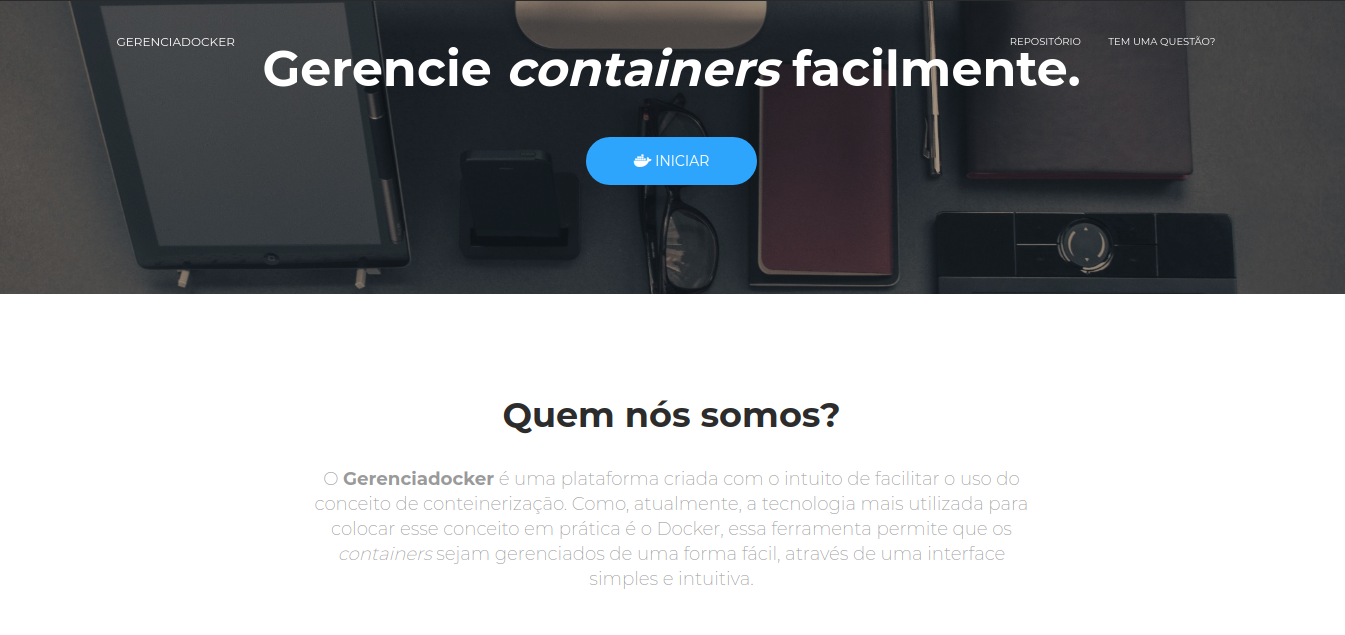
\includegraphics[width=1.0\textwidth]{./content/textuais/imagens/landing-page.png}}
    \label{fig:landing_page}
\end{figure}

Já a segunda, que é a tela de demonstração, é o local mais importante do sistema e pode ser acessado através do botão \aspas{Iniciar} exibido na figura \ref{fig:landing_page}. É nesse ambiente que o usuário criará sua \dockerNetwork{} e visualizará o estado atual de cada um dos \containers{} que a compõe. Além disso, também é possível interagir com cada \conteiner{} individualmente e utilizar opções como \aspas{Pausar}, \aspas{Retomar} ou \aspas{Excluir}, tal como pode ser visualizado na figura 3.

{\huge TELA DE DEMONSTRAÇÃO AQUI}








% PWA-------------------------------------------------------------------
\section{PWA}
\label{sec:pwa}

Os \textit{Progressive Web Apps}, que recentemente vem ganhando bastante popularidade e adeptos, podem ser definidos como \cite{Souza19} \aspas{uma aplicação \web{} com tecnologias que permitem termos a experiência de uso muito próxima da oferecida pelos \textit{mobile apps}}. Isso quer dizer, basicamente, que ao acessar um \textit{site}, o usuário terá a opção de adicionar um \aspas{atalho} para este no seu celular.

Porém, ao abrir esse atalho, a experiência para o utilizador será de estar utilizando um aplicativo nativo, como se tivesse \aspas{instalado o \textit{site}} em seu dispositivo. Isso porque ele não verá uma barra exibindo a \textit{URL} que está sendo acessada e, além disso, funções nativas do celular - como acesso à câmera, geolocalização, aos contatos e \textit{push notifications} - estarão em pleno funcionamento. Esse tipo de solução tem sido testada e utilizada por grandes empresas como Uber, Twitter e Facebook, por exemplo, em virtude de algumas vantagens que ela apresenta sobre os \textit{apps} nativos, principalmente em dois pontos: custos e engajamento do cliente.


Primeiramente, no quesito despesas, utilizar um \textit{PWA} permite que, com poucas alterações no site da empresa, ela disponibilize um \aspas{aplicativo} - o que economiza tempo de desenvolvimento e, consequentemente, dinheiro. Em segundo lugar, geralmente os \textit{PWAs} são mais rápidos, ocupam menos espaço de armazenamento no dispositivo e, em casos reais, ficou comprovado que a facilidade em obter esse \textit{app} gera mais conversão de clientes, conforme \cite{Souza19} \aspas{o Flipkart que é o maior e-commerce da Índia, eles decidiram fazer uma experiência mobile através de uma PWA e aumentaram a sua conversão em 70\%}.

Para resumir, sempre que deseja-se criar uma experiência agradável para o usuário, de forma rápida e com poucos custos, não sendo necessário implementar funcionalidades demasiadamente robustas, um \textit{PWA} é a melhor opção. No caso desse projeto, portanto, que se enquadra perfeitamente nessas características, o grupo considerou essa como sendo a tecnologia ideal para criarmos um aplicativo para este projeto.


\subsection{O Aplicativo}
\label{subsec:o_aplicativo}

Para tornar a solução ainda mais completa e próxima das necessidades do usuário, o grupo decidiu fazer um \textit{app} simples (utilizando a tecnologia citada no subcapítulo \ref{sec:pwa}) que irá listar todas as ocorrências de falhas nos \containers{}, além de disparar uma \textit{push notification} na tela do usuário. O objetivo principal deste aplicativo é servir como uma fonte de consulta para o usuário responsável pelo funcionamento da rede de \containers{}.

Isso porque, em virtude de relacionar-se com diversas variáveis (velocidade da rede, infraestrutura, tamanho das equipes, entre outras), é possível que esse tipo de rede apresente pequenas falhas com o decorrer do tempo. Como é de conhecimento de todos, o profissional moderno precisa, além de realizar várias tarefas em paralelo, contar com uma certa mobilidade e, portanto, não seria agradável que um colaborador precisasse monitorar a tela do sistema em tempo integral para identificar quando ocorresse um problema.

Em razão disso, era necessário chamar a atenção dos responsáveis por manter a rede funcionando de alguma forma. Analisando as tecnologias disponíveis nos dias de hoje, chegou-se ao consenso que uma notificação no celular é, provavelmente, um dos melhores meios de chamar a atenção de alguém. Na imagem abaixo, é possível visualizar a interface da versão final do aplicativo:

{\huge IMAGEM DA PWA AQUI}                      % Descrição da Implementação
    % CRONOGRAMA-------------------------------------------------------------------

\chapter{CRONOGRAMA}
\label{chap:cronograma}

\begin{figure}[!htb]
    \centering
    \caption{Cronograma}
    \frame{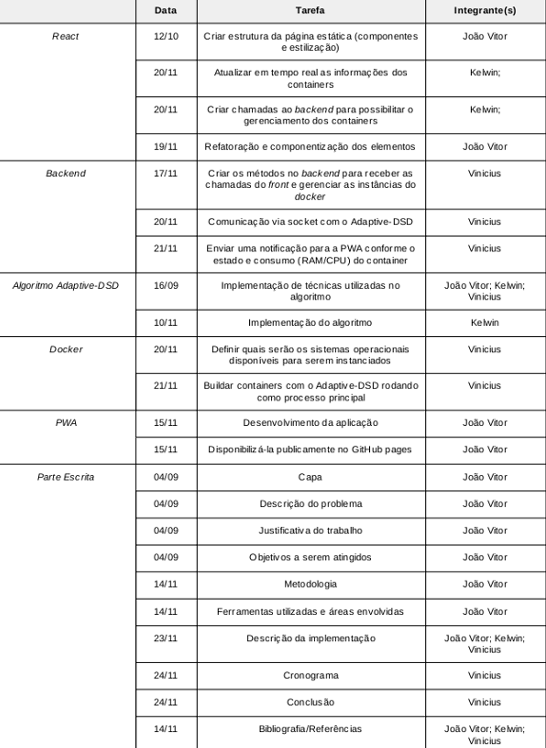
\includegraphics[width=0.9\textwidth]{./content/textuais/imagens/cronograma.png}}
    \label{fig:cronograma}
\end{figure}                                   % Cronograma Efetivo
    % CONCLUSÃO-------------------------------------------------------------------
\chapter{CONCLUSÃO}
\label{chap:conclusao}


% Desenvolver um sistema é um trabalho que vai muito além de programá-lo, e dentre todas as suas etapas, nós daremos enfâse a uma em específico, a arquitetura do sistema

% Um desenvolvedor deve ter habilidades que vão além da programação, dominar múltiplas áreas de conhecimento é praticamente obrigatório, pois é necessário para ter controle de suas soluções, até por que uma solução (dependendo de sua complexidade) exige que inúmeras tecnologias e conhecimentos sejam interligados, que no final de fato solucionarão um problema.

% Esse tipo de exercício exige dos alunos conhecimentos que serão necessários no mercado de trabalho, pois um desenvolvedor deve ser versátil, eficiente e tem a obrigação de dominar sua soluções.

% O trabalho possui uma proposta muito interessante, pois ele faz com que o aluno pense em um problema real e busque solucioná-lo. É notório que solucionar um problema exige que múltiplas tecnologias e áreas de conhecimento sejam interligadas, até porque criar uma solução vai muito além de programá-la.

% Existe uma grande aproximação desse exercício acadêmico com o que o mercado de trabalho exige, principalmente pelo fato de estarmos tentando solucionar um problema real. Vale ressaltar que esse realismo foi um grande motivador durante a realização do projeto.

O trabalho possui uma proposta muito interessante, pois ele faz com que o aluno pense em um problema real e busque solucioná-lo. Com base nisso e também na notoriedade de que solucionar um problema exige que os alunos interliguem múltiplas tecnologias e áreas de conhecimento, ele provou-se muito relevante para todos os membros do grupo.

Notou-se uma grande aproximação desse exercício acadêmico com o que o mercado de trabalho exige, principalmente pelo fato de induzir os alunos a solucionar um problema real, o que mostrou-se muito benéfico para os membros do grupo, pois acabou motivando a todos. Ainda dentro desse paralelismo com o mercado de trabalho, o maior benefício dentre os pontos positivos, pode-se dizer, é aprender a criar uma solução, passando por todas as etapas de construção da mesma e adotando métodos para que as entregas e a distribuição de tarefas sejam organizadas.

Outro ponto muito importante que deve ser mencionado, é a possibilidade de pôr em prática muito do que foi aprendido em outras disciplinas e não havia sido implementado. Vale destacar, novamente, que isso só é possível devido à proposta do trabalho, onde é dada a liberdade para que o aluno escolha quais serão as áreas que ele deseja utilizar. Inclusive, esse ponto pode ser muito bem aproveitado, pois incentiva que o aluno aprofunde-se ainda mais em alguma das áreas da Ciência da Computação, permitindo uma enorme extração de ideias para o Trabalho de Conclusão de Curso ou até mesmo para áreas de atuação que ele possa trabalhar.

A maior dificuldade do grupo, no entanto, foi cumprir o cronograma esboçado na proposta entregue ao professor, sendo que alguns prazos acabaram não sendo respeitados. Todos esses atrasos ocorreram influenciados por fatores externos como, por exemplo, tarefas que tiveram que ter uma prioridade maior naquele período de tempo. Porém, é importante enfatizar que o cronograma foi importante para a organização de tarefas, pois ele proporcionou uma visão geral do projeto que foi crucial na distribuição das mesmas e, com isso, todas as decisões permearam o cronograma inicialmente montado.

Correndo o risco de ser redundante, gostaríamos de fortalecer que a proposta do trabalho é extremamente válida e de fato agrega muito conhecimento para os alunos, como anteriormente mencionado, pois existe um paralelismo muito interessante com as exigências do mercado de trabalho atual. Não existe nenhum tipo de crítica quanto ao formato ou modelo propostos para sua execução. Por fim, entregamos o projeto com uma sensação de dever cumprido, pois atingimos todos os objetivos que foram inicialmente definidos com a ajuda do professor.                   		            % Conclusão

    \postextual

    % INSERE ELEMENTOS PÓS-TEXTUAIS
    % REFERÊNCIAS------------------------------------------------------------------

% Carrega o arquivo "referencias.bib" e extrai automaticamente as referências citadas
{\renewcommand{\contentsname}{MAC}}
\bibliography{./gerenciadocker}
\bibliographystyle{abntex2-alf} % Define o estilo ABNT para formatar a lista de referências
% OBSERVAÇÕES------------------------------------------------------------------
% Este arquivo não precisa ser alterado.           			        % Referências


\end{document}
% <ENCERRA>
%   Conteúdo do Documento: base teórica.
% </ENCERRA>